\section{Anhang}
\subsection{Schachbrett zur Kamerakalibrierung}\label{sec:schachPDF}

\begin{figure}[H] 
	\center 
	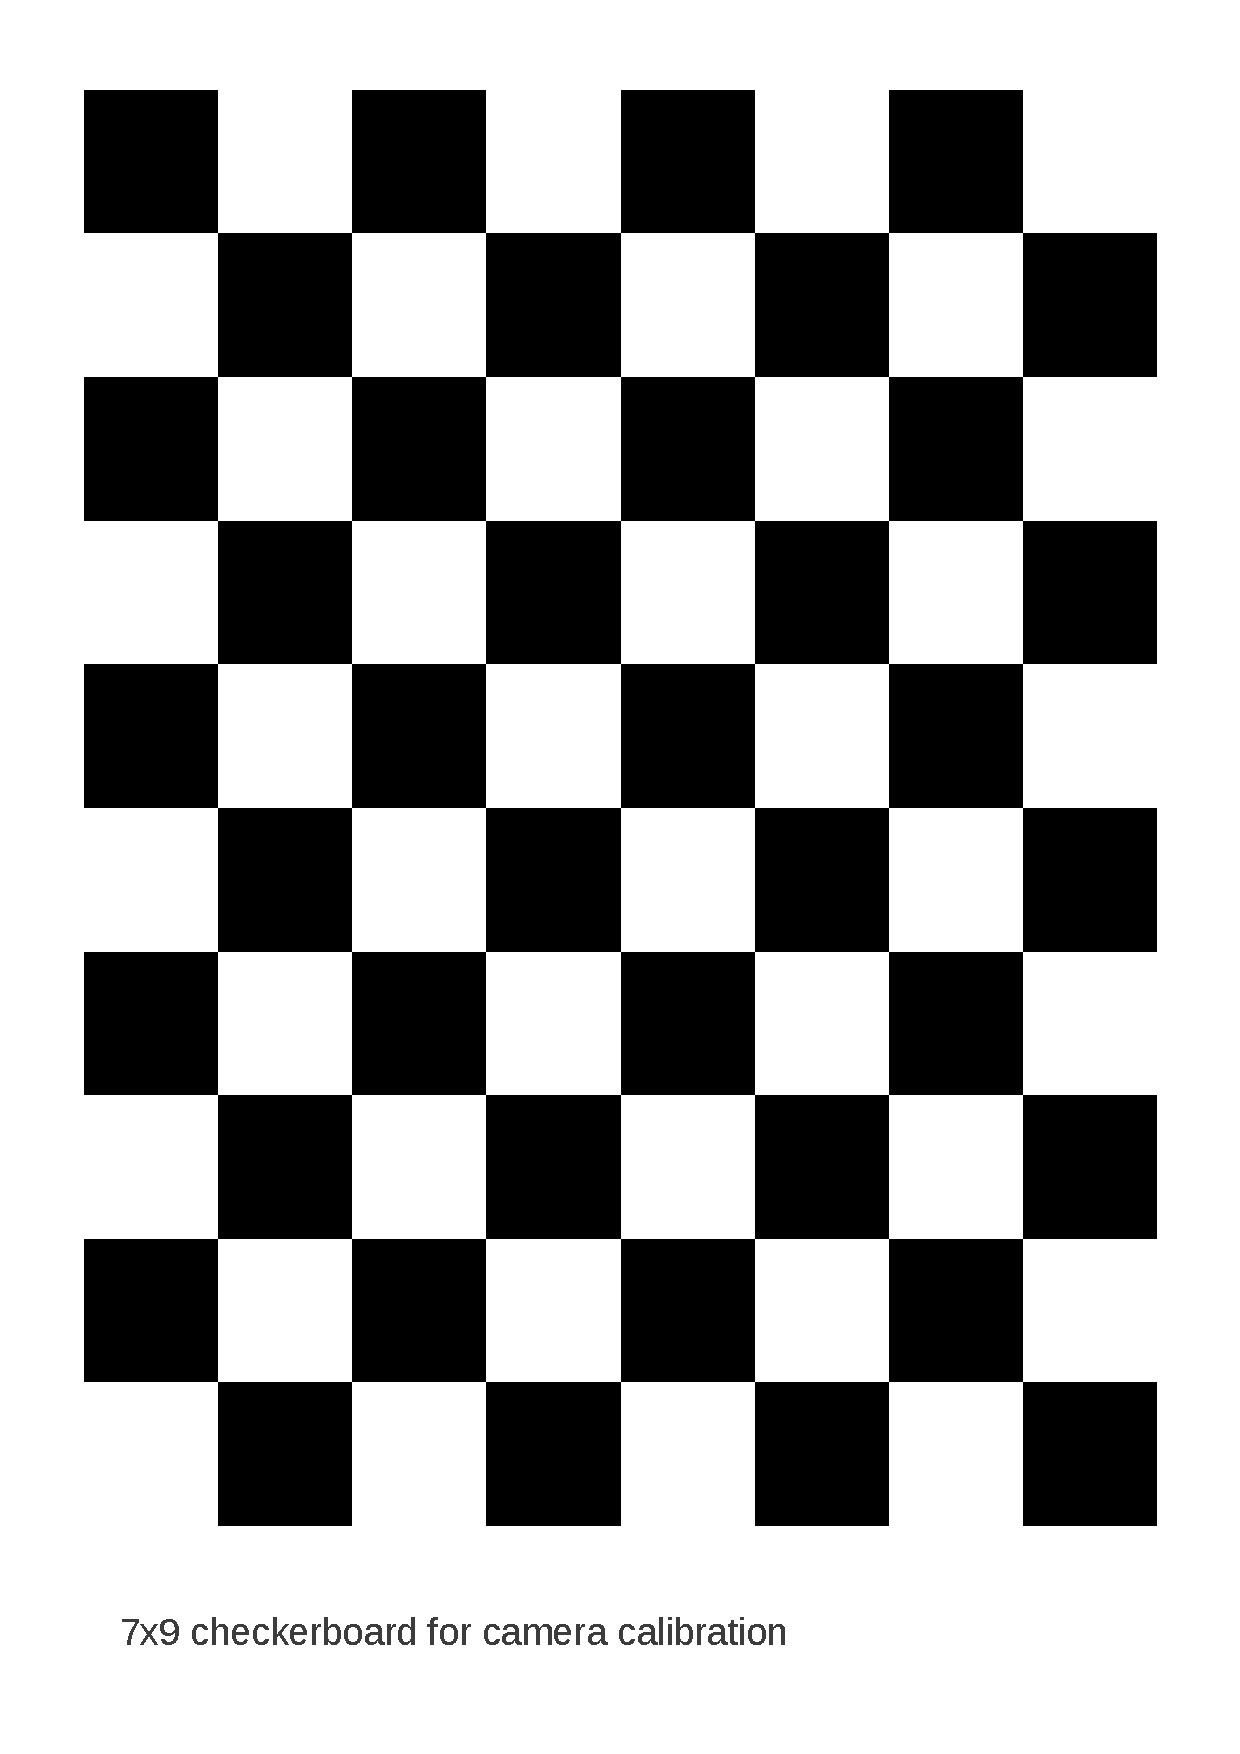
\includegraphics[scale = 0.6]{Bilder/camera-calibration-checker-board_9x7.pdf}			
	\caption{Um den Faktor 0.6 skaliertes Schachbrett zur Kamerakalibrierung. \\ Download: \url{http://www.mrpt.org/downloads/camera-calibration-checker-board_9x7.pdf}}
	\label{fig:schachPDF}
\end{figure}

\subsection{\emph{MArC} ReadMe-Datei}\label{sec:readMe}
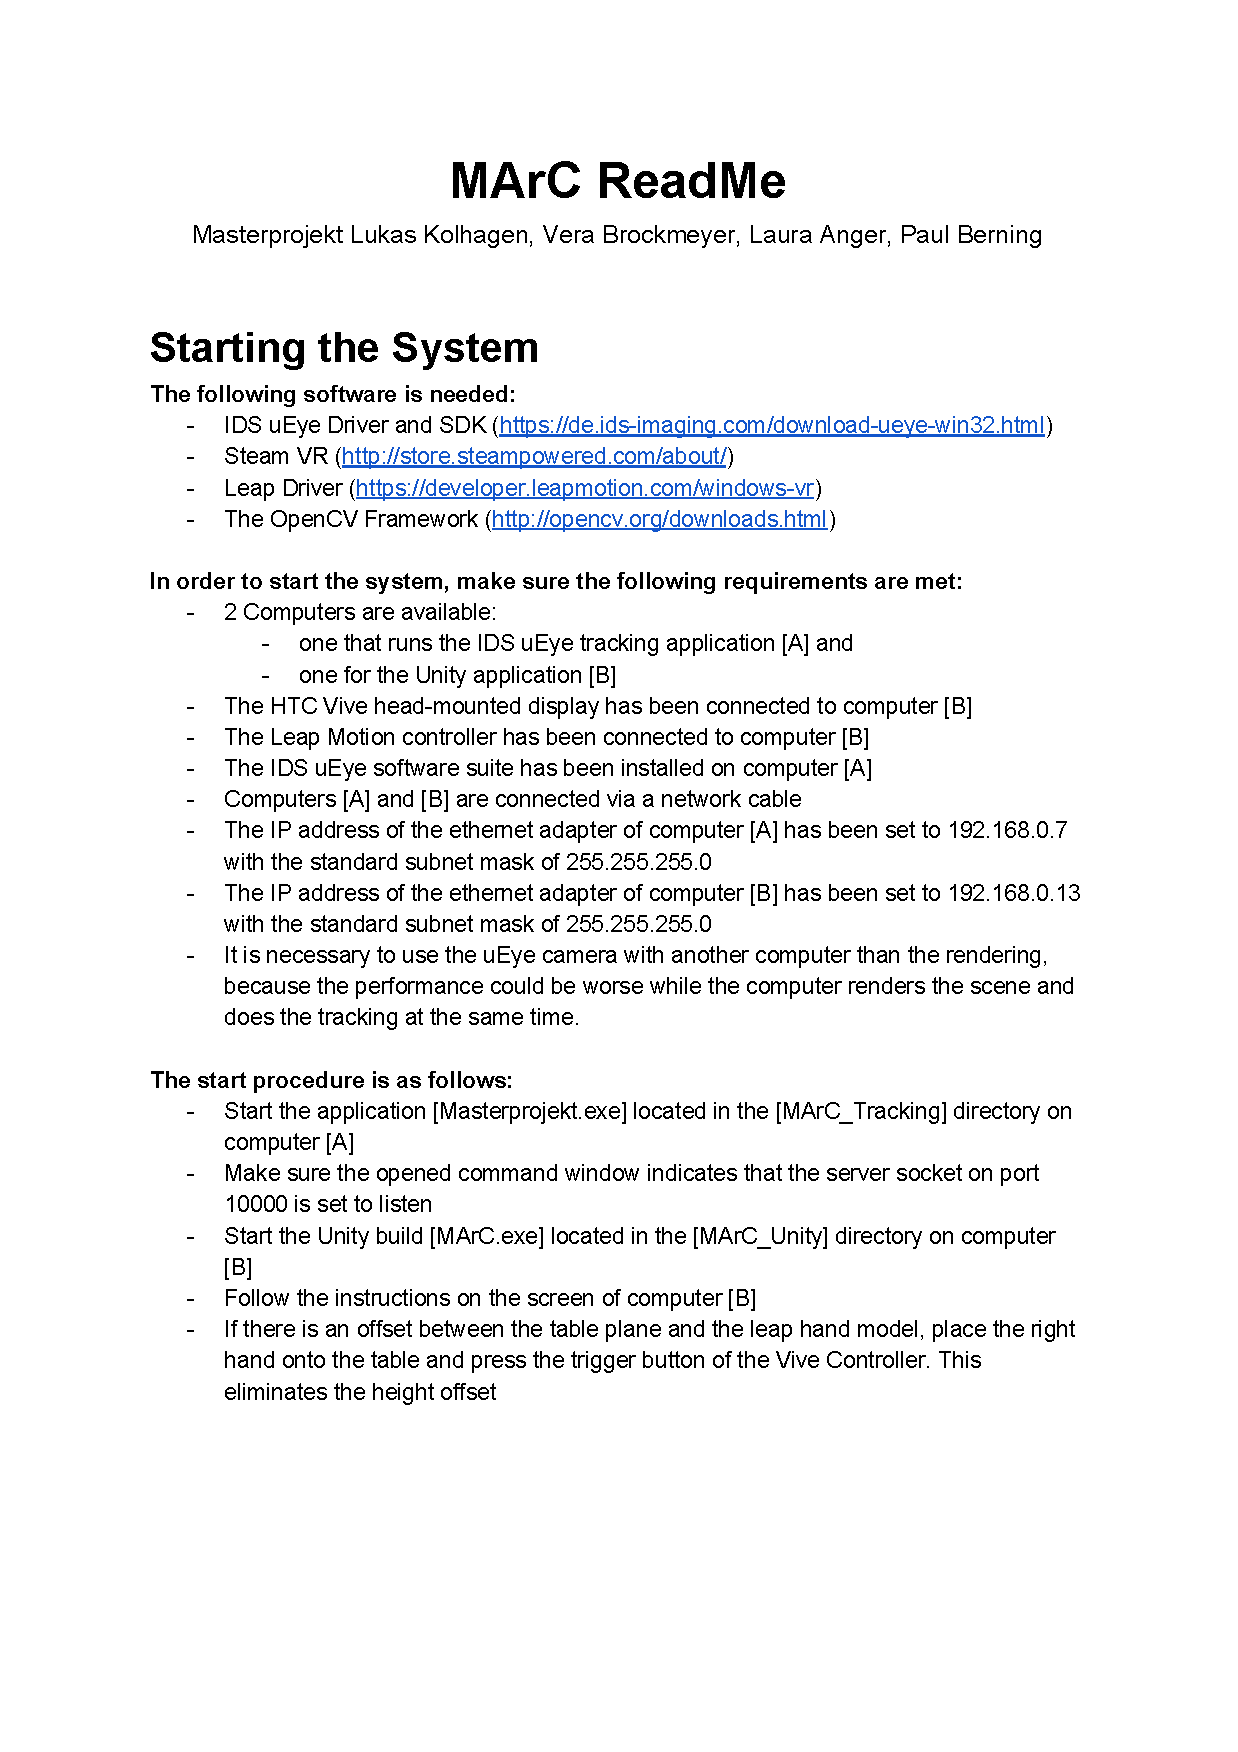
\includepdf[pages=-]{kapitel/anhang/ReadMe.pdf} 

\subsection{\texttt{startTCPServer()}-Methode}
\lstinputlisting[title=\lstname, caption={\texttt{startTCPServer()}-Methode in \texttt{TCP.cpp}}, label=lst:startTCPServer, language={C++}, linerange=22-77, firstnumber=22]{Quellcode/TCP.cpp}

\subsection{\texttt{getPointerOfMarkerVec()}-Methode}
\lstinputlisting[title=\lstname, caption={\texttt{getPointerOfMarkerVec()}-Methode in \texttt{TCP.cpp}}, label=lst:getPointerOfMarkerVec, language={C++}, linerange=131-164, firstnumber=131]{Quellcode/TCP.cpp} 

\subsection{\texttt{interpretTCPMarkerData()}-Methode}
\lstinputlisting[title=\lstname, caption={\texttt{interpretTCPMarkerData()}-Methode in \texttt{readInNetWorkData.cs}}, label=lst:interpretData, language={[Sharp]C}, linerange=141-174, firstnumber=141]{Quellcode/readInNetworkData.cs}
\newpage
\begin{figure}[htbp]
	\centering
	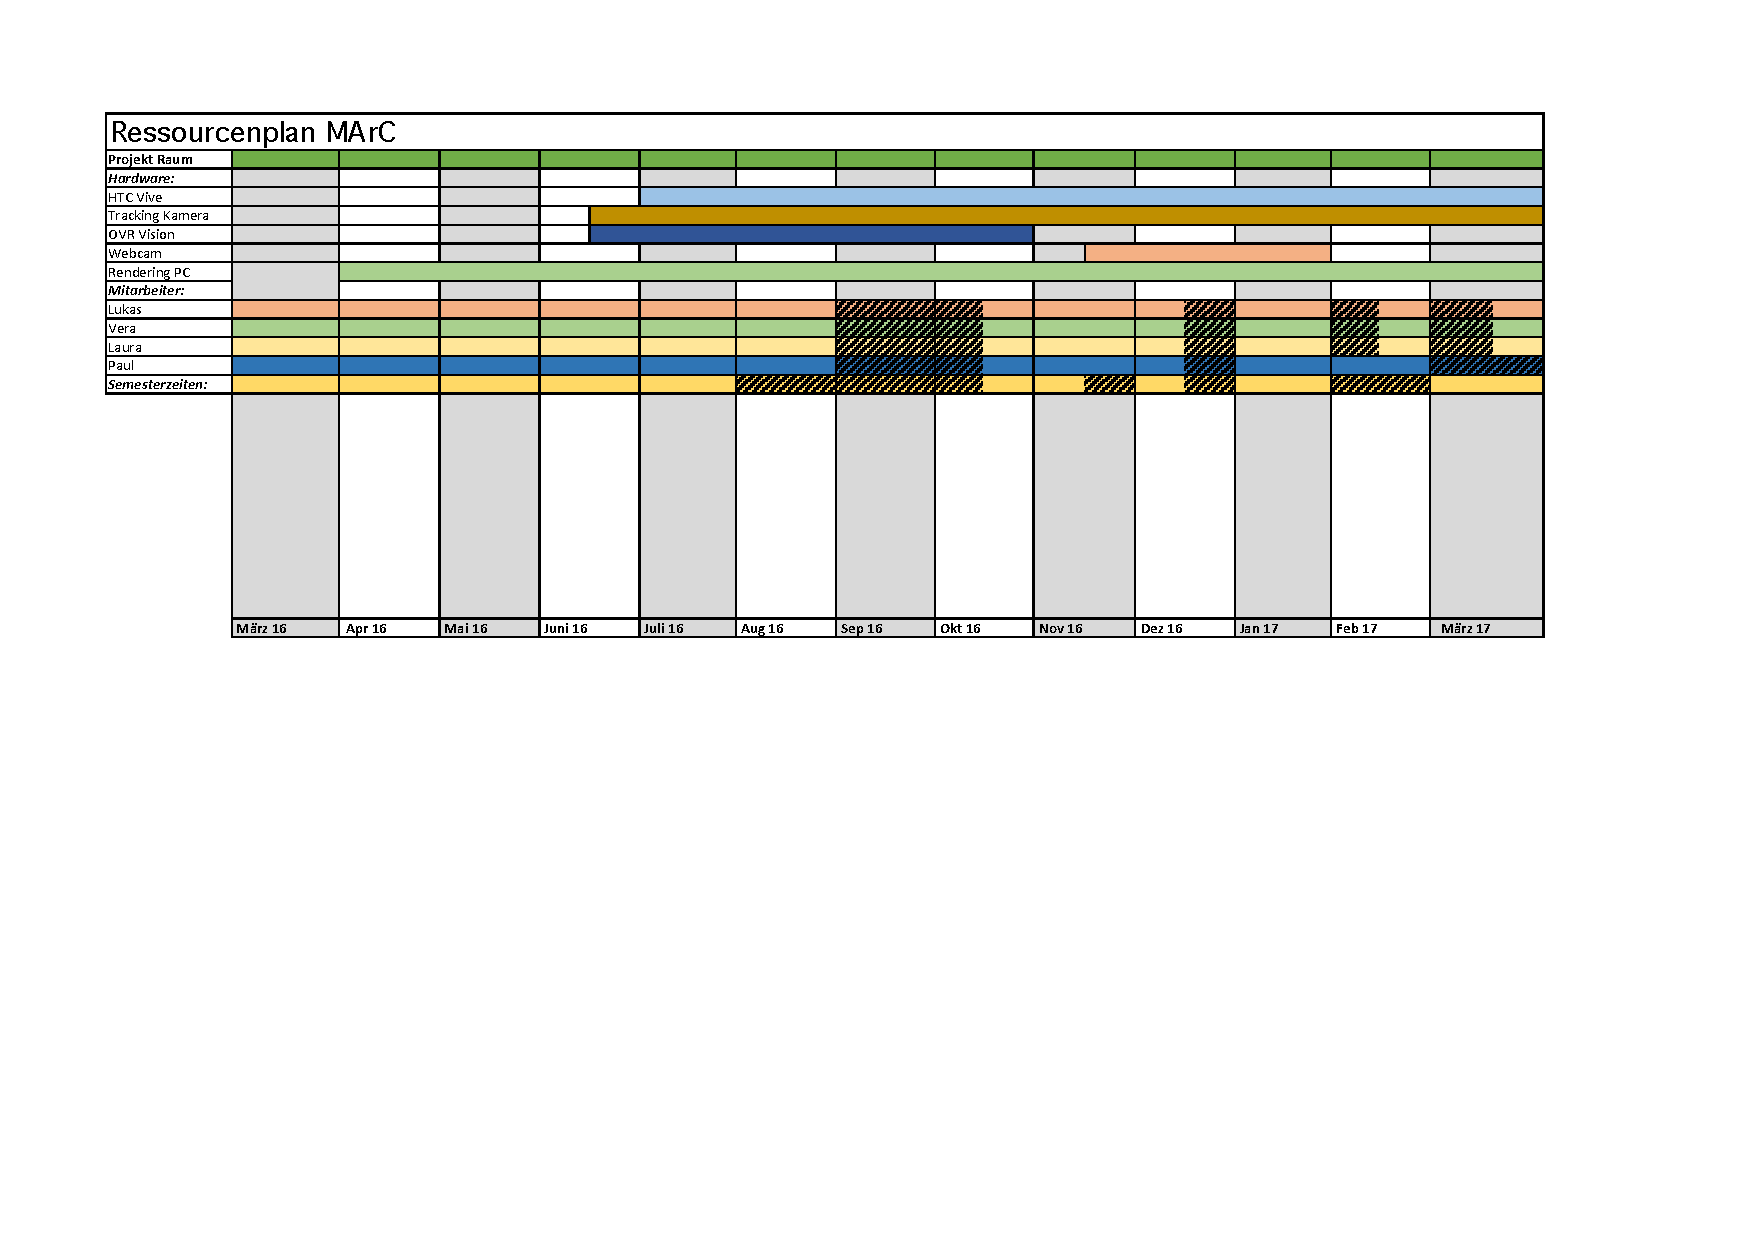
\includegraphics[angle=90,scale=.9, trim=1cm 1cm 3cm 3 cm]{kapitel/anhang/Kapazitaetsplan.pdf}
	
	 \caption{Ressourcenplan von \textit{MArC} in tabellarischer Form.}
	\label{fig:ressourcenplan}
\end{figure}

\begin{figure}[htbp]
	\centering
	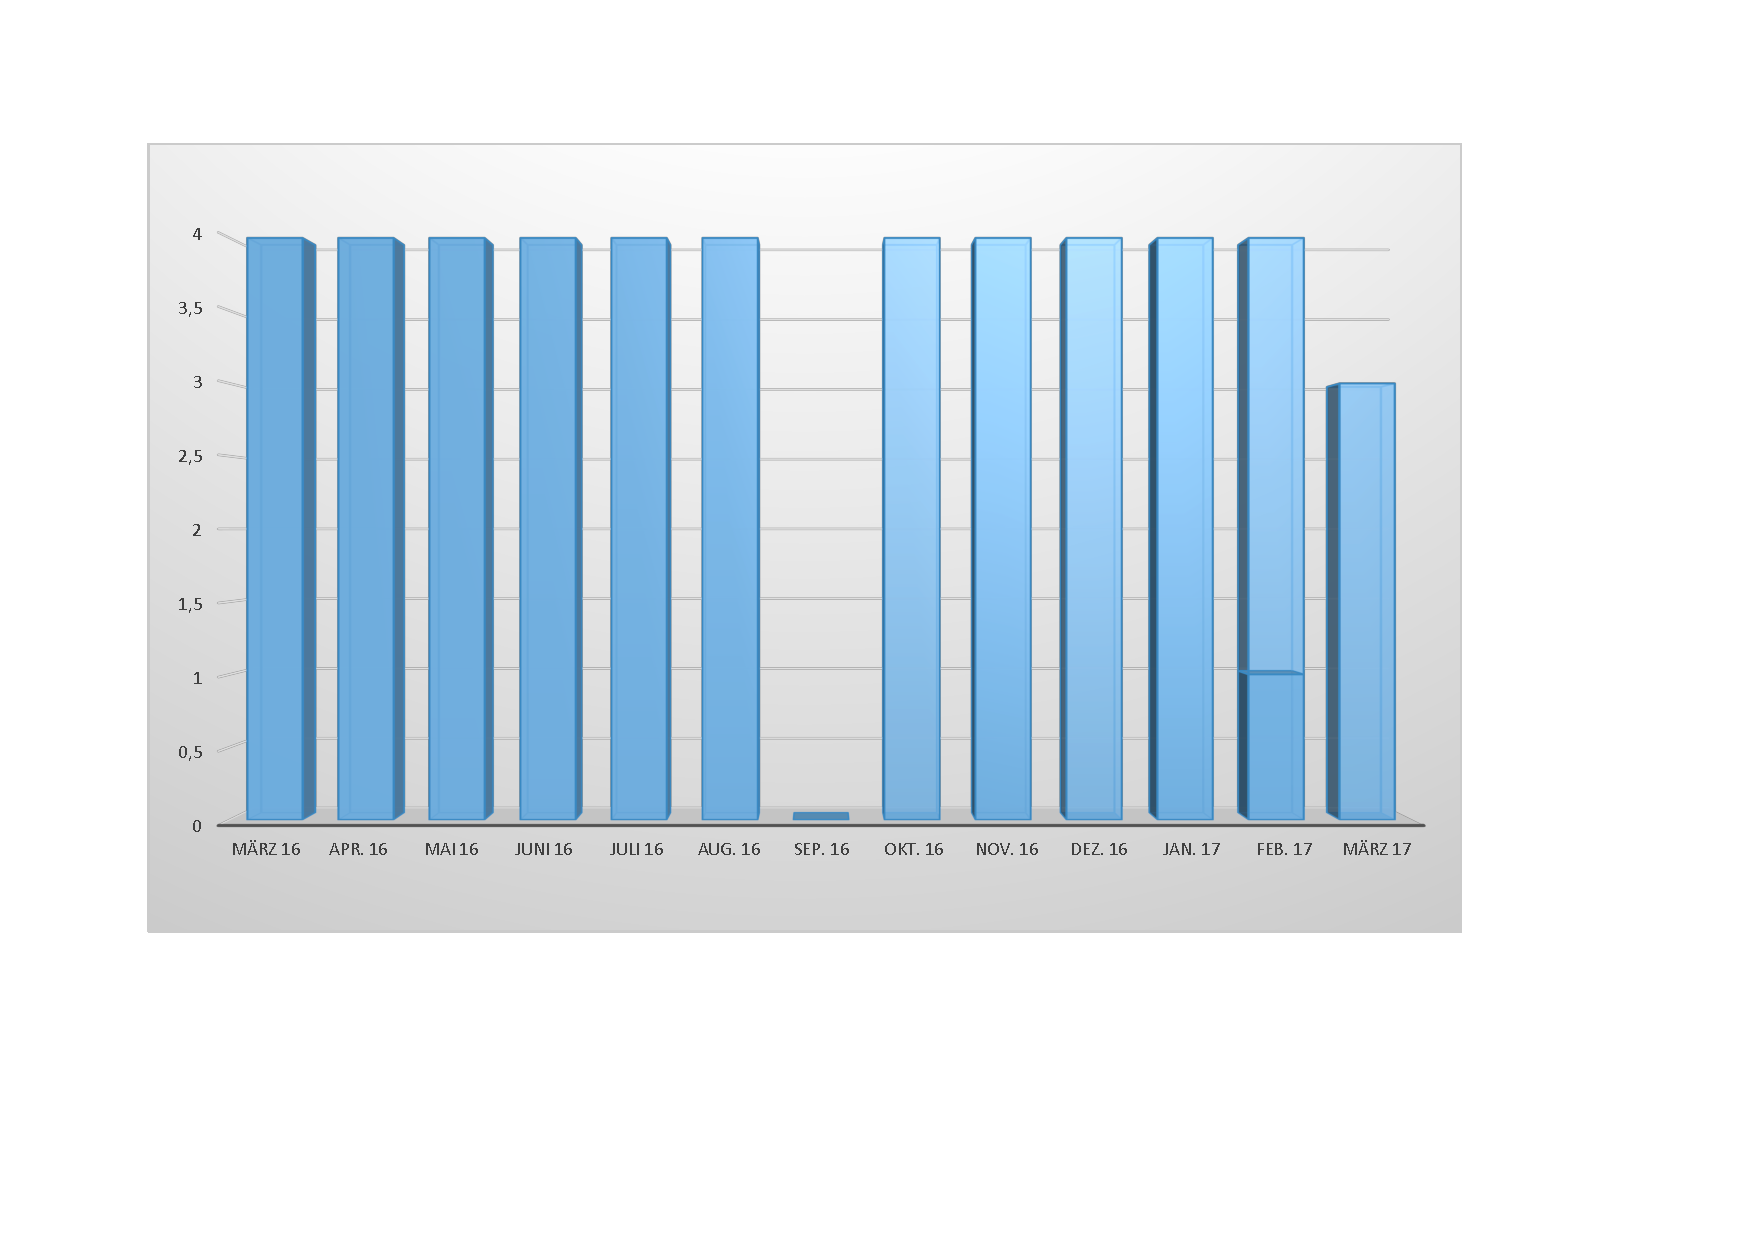
\includegraphics[angle=90,scale=.9, trim=1cm 1cm 3cm 3 cm]{kapitel/anhang/Kapazitaetsplan2.pdf}
	
	 \caption{Mitarbeiterressourcenplan von \textit{MArC} als Diagramm.}
	\label{fig:ressourcenplanDiagramm}
\end{figure}

\newpage
\begin{figure}[htbp]
	\centering
	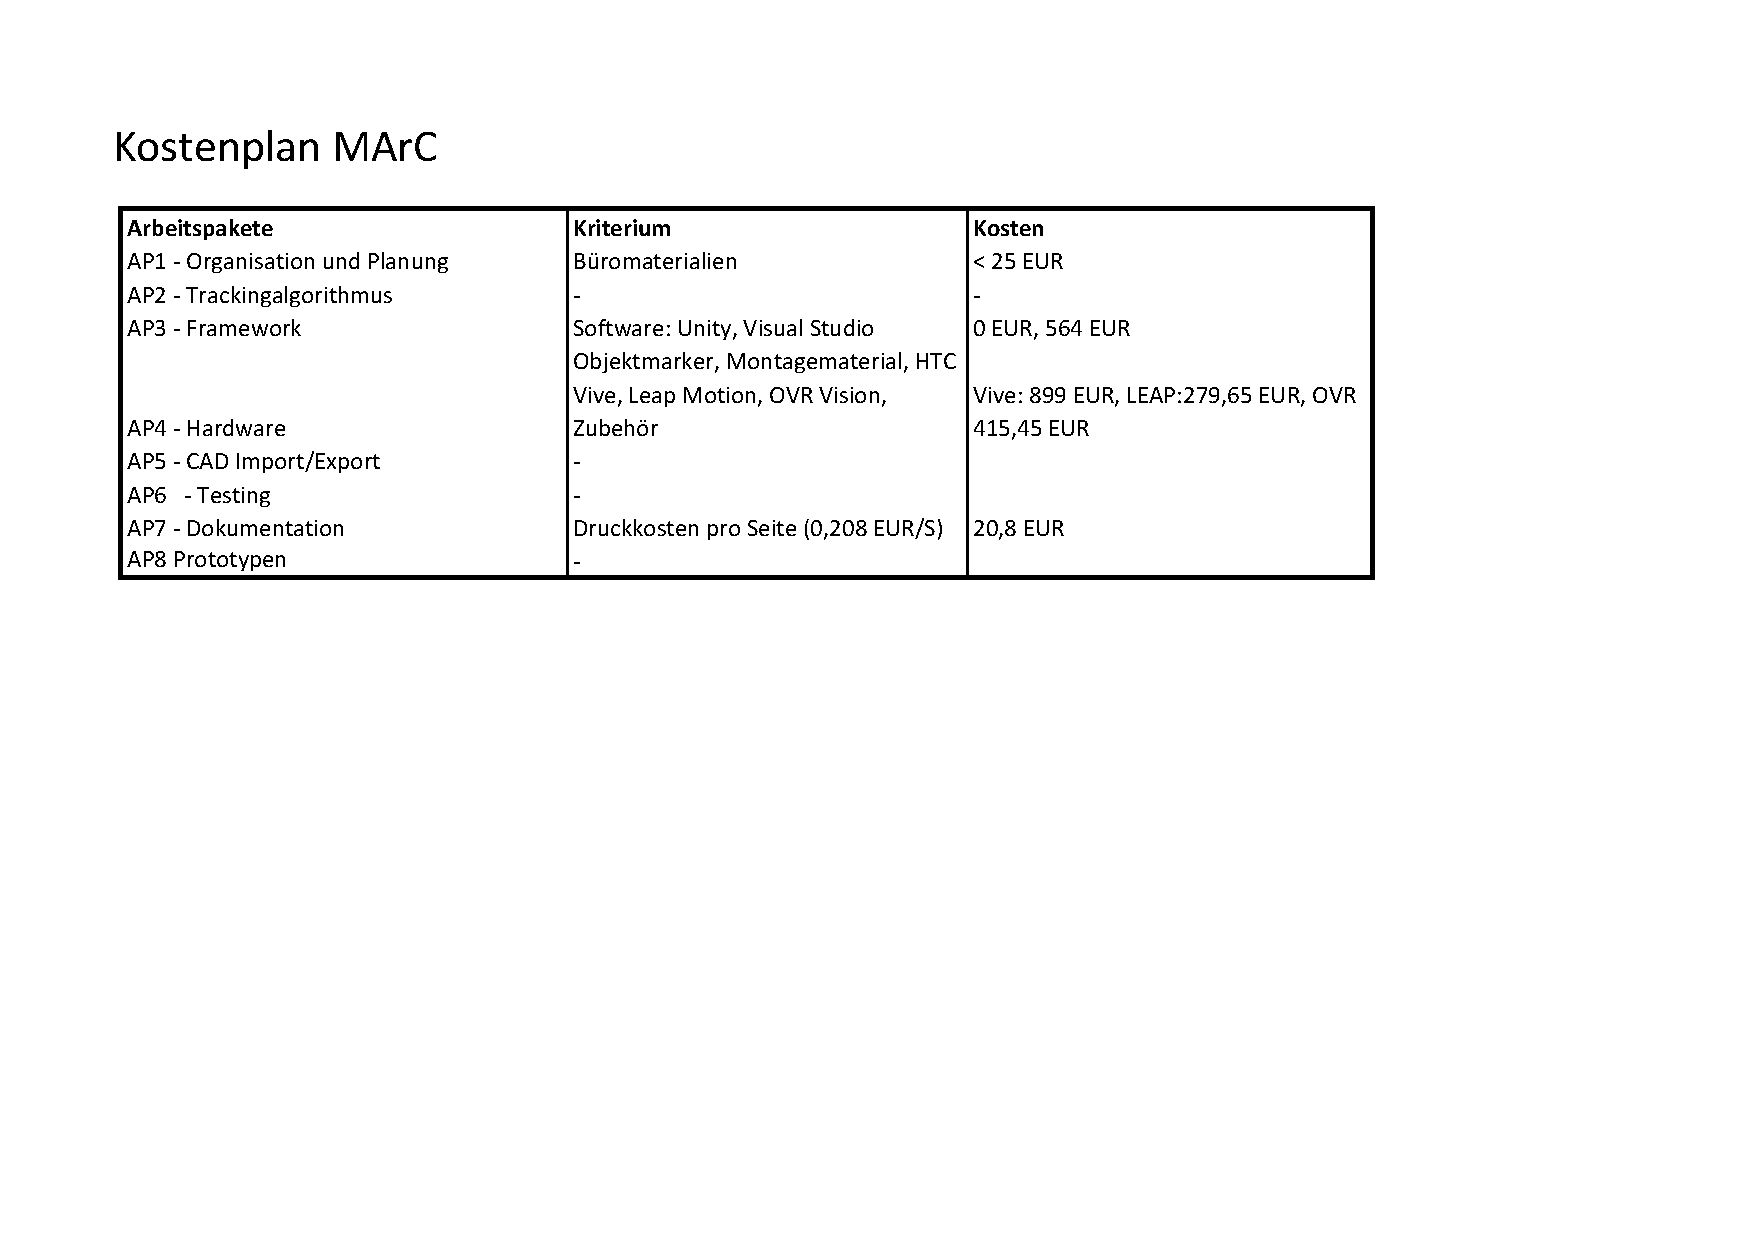
\includegraphics[angle=90,scale=.9, trim=1cm 1cm 3.5cm 1 cm]{kapitel/anhang/Kostenplan.pdf}
	 \caption{Kostenplan von \textit{MArC}.}
	\label{fig:kostenplan}
\end{figure}
\newpage

\begin{figure}[htbp]
	\centering
	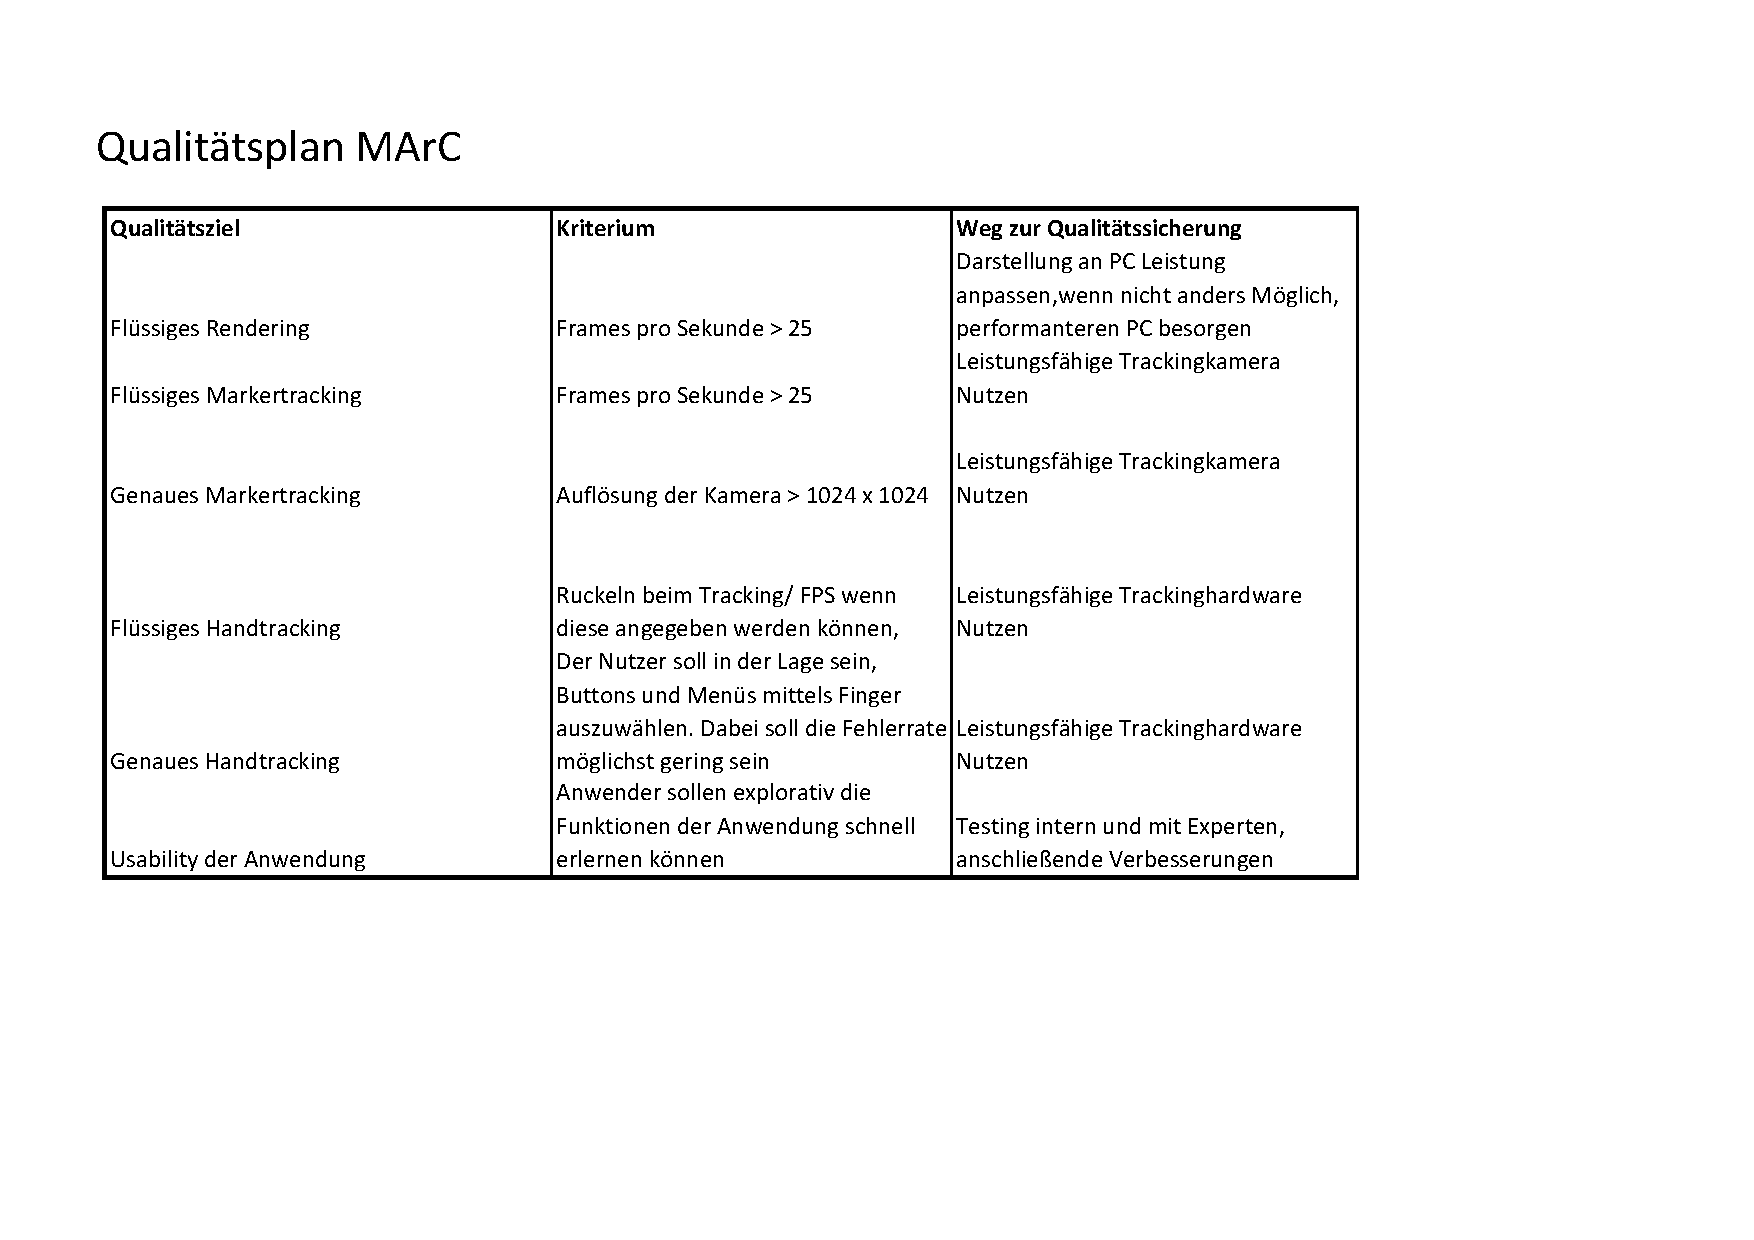
\includegraphics[angle=90,scale=.9, trim=1cm 1cm 3.5cm 1 cm]{kapitel/anhang/Qualitaetsplan.pdf}
	 \caption{Qualitätsplan von \textit{MArC}.}
	\label{fig:qualitaetsplan}
\end{figure}
\newpage

\begin{figure}[htbp]
	\centering
	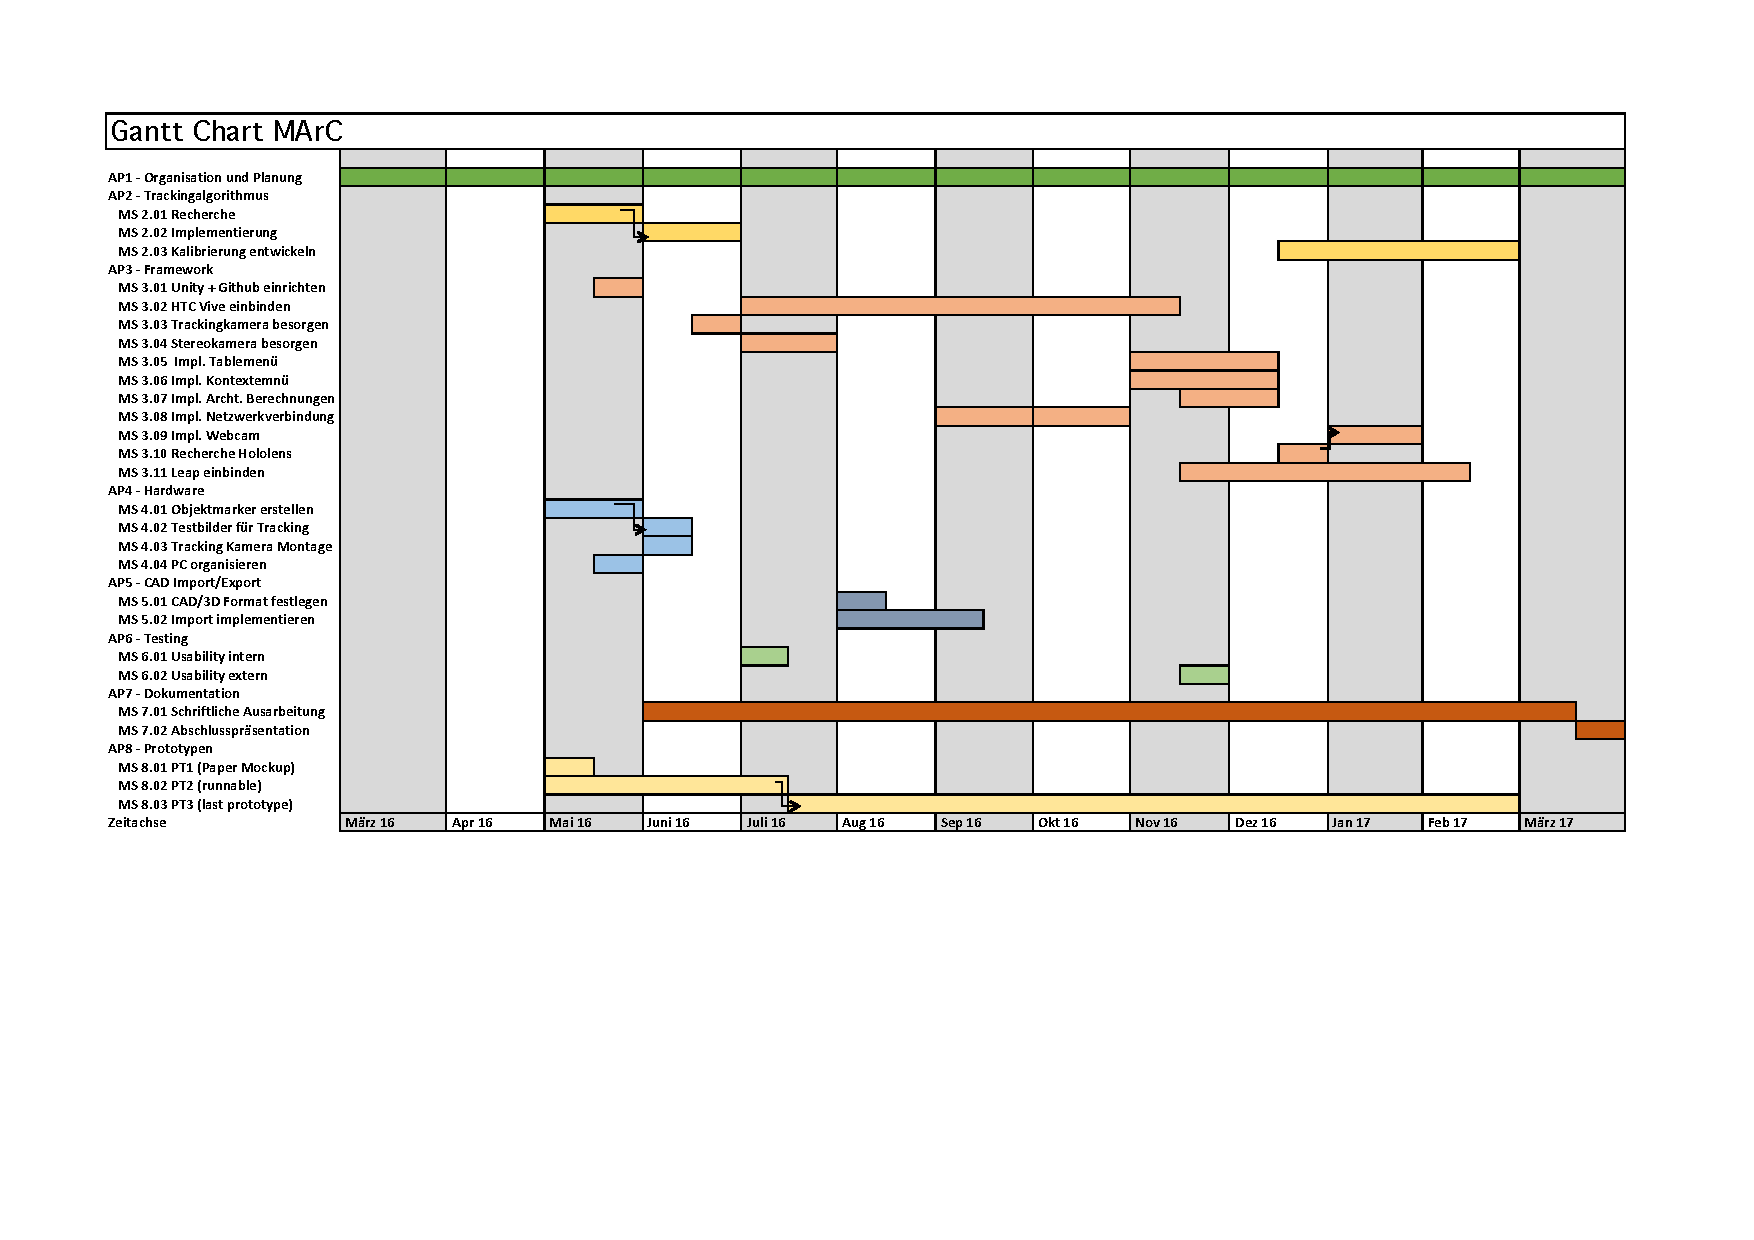
\includegraphics[angle=90,scale=.8, trim=1cm 1cm 3.5cm 1 cm]{kapitel/anhang/GanttChart.pdf}
	 \caption{Gantt Chart von \textit{MArC}.}
	\label{fig:ganttchart}
\end{figure}
\newpage

\begin{figure}[htbp]
	\centering
	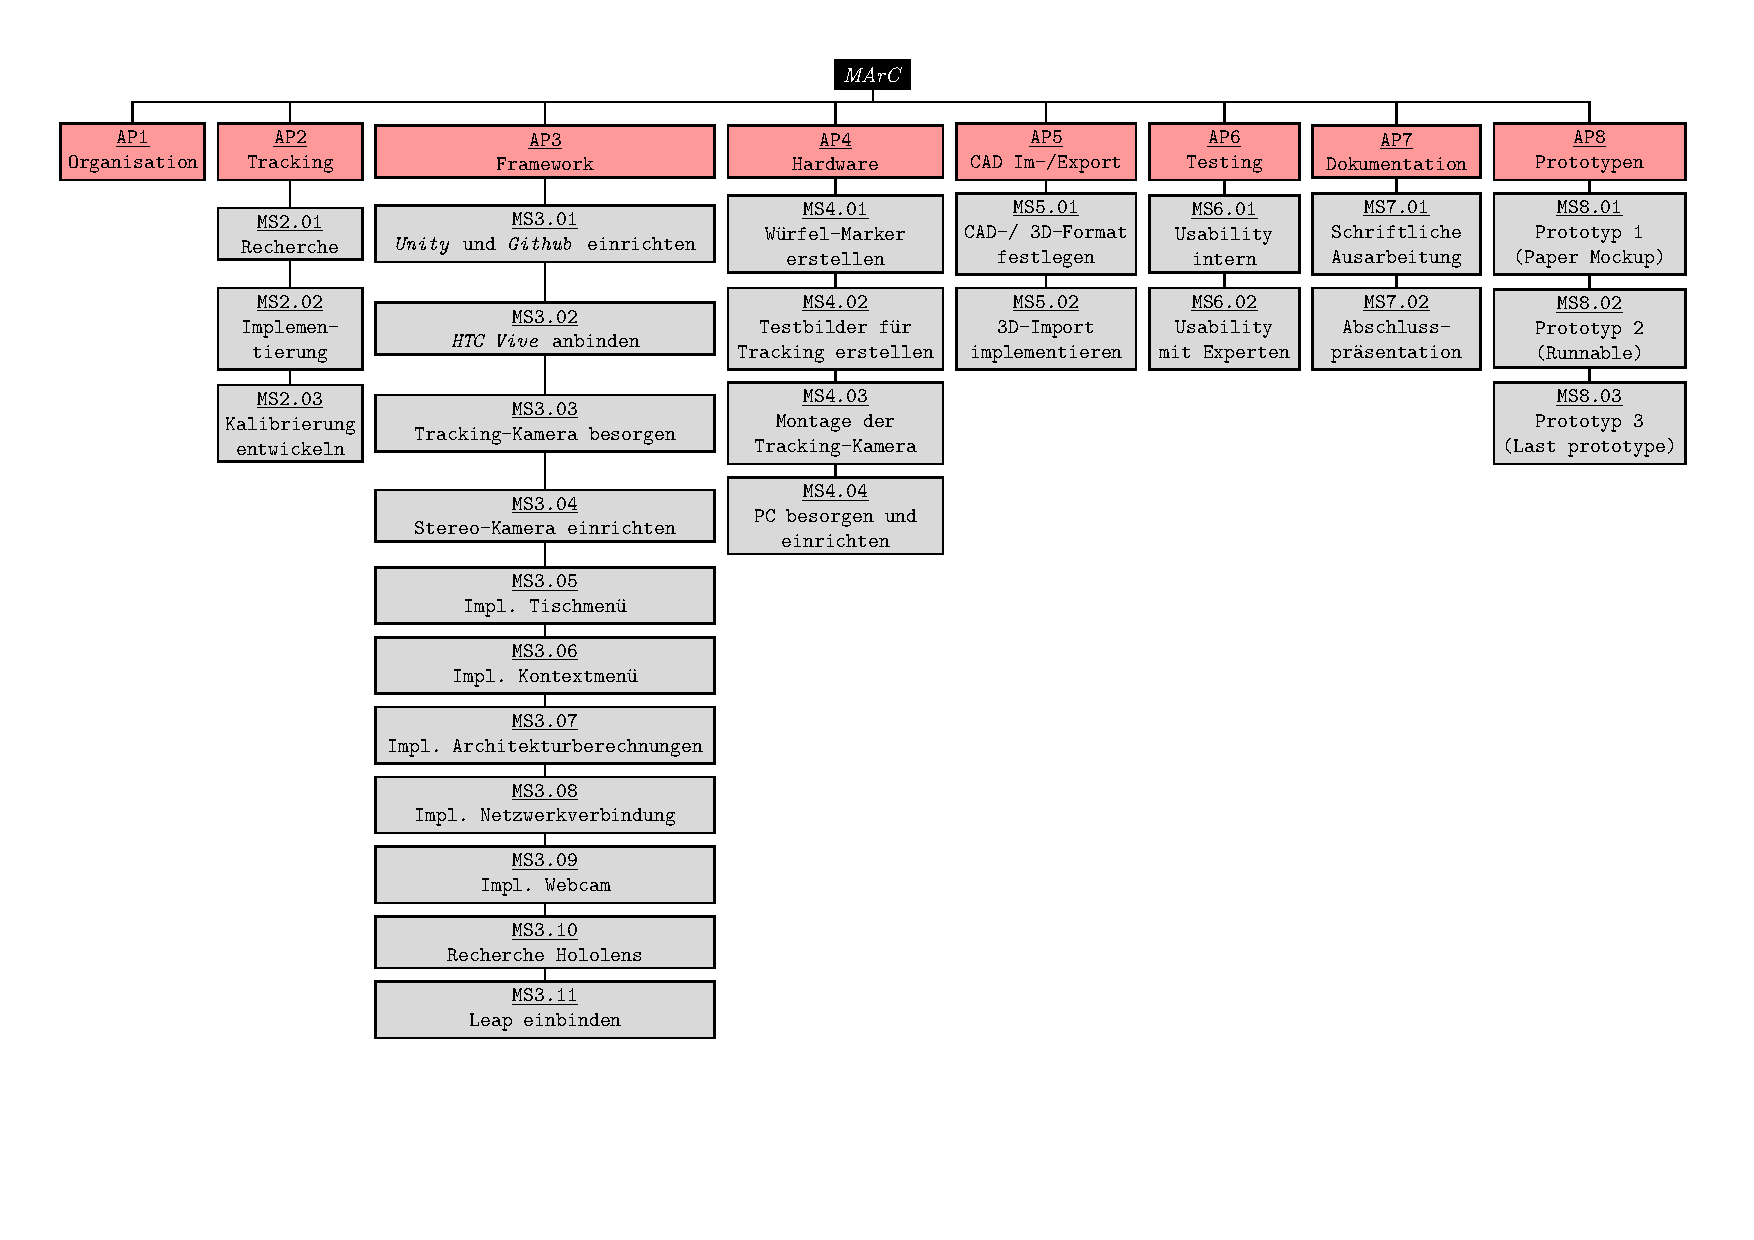
\includegraphics[angle=90,scale=.9, trim=1cm 1cm 3.5cm 1 cm]{kapitel/anhang/MP_Strukturplan.pdf}
	 \caption{Projekt Strukturplan von \textit{MArC}.}
	\label{fig:psp}
\end{figure}
\newpage

%\subsection{\texttt{runCalibWithChessboard()}-Methode}
%\lstinputlisting[title=\lstname, caption={\texttt{runCalibWithChessboard()}-Methode in \texttt{calibWithChessboard.cpp}}, label=lst:runCalibWithChessboard, language={[Sharp]C}, linerange=146-349, firstnumber=146]{Quellcode/calibWithChessboard.cpp}

%\subsection{\texttt{runCalibration()}-Methode}
%\lstinputlisting[title=\lstname, caption={\texttt{runCalibration()}-Methode in \texttt{calibWithChessboard.cpp}}, label=lst:runCalibration, language={[Sharp]C}, linerange=71-103, firstnumber=71]{Quellcode/calibWithChessboard.cpp}


